\documentclass[11pt,fancy]{elegantbook}

\usepackage{tikz-cd}
\usepackage{cancel}
\providecommand{\tq}{\mid}
\providecommand{\N}{\mathbb{N}}
\providecommand{\Z}{\mathbb{Z}}
\providecommand{\Q}{\mathbb{Q}}
\providecommand{\R}{\mathbb{R}}
\providecommand{\C}{\mathbb{C}}
\providecommand{\H}{\mathcal{H}}
\providecommand{\Im}[1]{Im(#1)}
\providecommand{\Re}[1]{Re(#1)}
\providecommand{\conjugate}[1]{\bar{#1}}
\providecommand{\pescalar}[2]{\langle #1,#2 \rangle}
\providecommand{\braket}[2]{\left\langle#1\mid#2\right\rangle}
\providecommand{\bra}[1]{\left\langle#1\right\rvert}
\providecommand{\ket}[1]{\left\lvert#1\right\rangle}
\providecommand{\so}{\Rightarrow}
\providecommand*{\circled}[1]{\tikz[baseline=(char.base)]{\node[shape=circle,draw,inner sep=2pt] (char) {#1};}}
\providecommand{\by}[1]{\overset{\fbox{\tiny #1}}{=}}
\providecommand{\maps}[3]{#1:#2\longrightarrow #3}
\providecommand{\coma}{,\thinspace}
\providecommand{\pari}[2]{(#1,\thinspace #2)}
\providecommand{\cartalocal}{(\mathcal{M}^n,\thinspace p,\thinspace U,\thinspace \varphi)\textmd{ una carta local}}
\providecommand{\doscartaslocales}{(\mathcal{M}^n\coma p\coma U\coma\varphi)\textmd{ y } (\mathcal{N}^m\coma q\coma
V\coma\psi)\textmd{ dos cartas locales}}
\providecommand{\indexdots}[3]{#1=#2,\ldots,#3}
\providecommand{\define}[2]{\textbf{#1}\label{def:#2}}
\providecommand{\avg}[1]{\left\langle#1\right\rangle}
\providecommand{\abs}[1]{\lvert#1\rvert}
\providecommand{\nor}[1]{\lVert#1\rVert}
\providecommand{\operatoravg}[3]{\left\langle#1|#2|#3\right\rangle}
\providecommand{\cinfinity}[1]{\mathscr{C}^\infty(#1)}
\providecommand{\mapsdef}[5]{ #1:\ #2 & \longrightarrow #3 \\ #4 & \longmapsto #5}
\providecommand{\glossarydef}[3]{\newglossaryentry{#1}{name={#2},description={#3}}\gls{#1}}
\providecommand{\lie}[2]{[#1\coma #2]}
\providecommand{\metrica}{\mathsf{g}}
\providecommand{\vec}[1]{\overrightarrow{#1}}
\newcommand{\set}[1]{\left\{#1\right\}}
\newcommand{\where}{\mathrel{}\middle|\mathrel{}}
\renewcommand*{\hbar}{{\mkern-1mu\mathchar'26\mkern-8mu\mathrm{h}}}
\renewcommand{\c}{\mathrm{c}}
\newcommand{\h}{\mathrm{h}}
\newcommand{\amplitud}{\mathrm{A}}
\newcommand{\longonda}{\lambda}
\newcommand{\frecuencia}{\nu}
\newcommand{\fase}{\alpha}
\newcommand{\frecuenciaangular}{\omega}
\newcommand{\longondaangular}{\mathrm{K}}
\newcommand{\periodo}{\mathrm{T}}
\newcommand{\energia}{\mathrm{E}}
\newcommand{\fuconda}{\Psi}
% Box color
\newcommand{\colorequation}[3]{\tcboxmath[on line,
    fonttitle=\small\sffamily,
    colbacktitle=#2!10!white,coltitle=#2!50!black,
    title=\small{#1},
    arc=0pt,outer arc=0pt,
    colback=#2!10!white,colframe=#2!50!black,
    boxsep=1pt,left=1pt,right=1pt,top=1pt,bottom=1pt,
    boxrule=0pt]{#3}}

% From mandi package
\newcommand{\usk}{\cdot}
\newcommand{\kilogram}{\mathrm{kg}}
\newcommand{\meter}{\mathrm{m}}
\newcommand{\second}{\mathrm{s}}
\newcommand{\inverse}{^{-1}}           % postfix -1
\newcommand{\tothetwo}{^2}             % postfix  2
\newcommand{\tothethree}{^3}           % postfix  3
\newcommand{\tothefour}{^4}            % postfix  4
\newcommand{\tento}[1]{10^{#1}}
\newcommand{\xtento}[1]{\times\tento{#1}}
%Constantes
\providecommand{\speedoflightsymbol}{\c}
\providecommand{\speedoflightvalue}{2.99792458\times10^{8}}
\providecommand{\speedoflightounits}{\meter\usk\second\inverse}
\providecommand{\plancksymbol}{\h}
\providecommand{\planckvalue}{6.62607015\times10^{-34}}
\providecommand{\planckunits}{\kilogram\usk\meter\tothetwo\usk\second\inverse}
\providecommand{\planckbarsymbol}{\hbar}
\providecommand{\planckbarvalue}{1.054571817\times10^{-34}}
\providecommand{\planckbarunits}{\kilogram\usk\meter\tothetwo\usk\second\inverse}
%Unidades
\providecommand{\mass}[1]{#1\ \kilogram}
\providecommand{\espacio}[1]{#1\ \meter}
\providecommand{\velocity}[1]{#1\ \meter\usk\second\inverse}
\providecommand{\momento}[1]{#1\ \kilogram\usk\meter\usk\second\inverse}

\newcommand\ct[1]{\text{\rmfamily\upshape #1}}

\title{Apuntes en mecánica cuántica}
\subtitle{La visión de un matemático}

\author{Francisco Costa Cano}
\bioinfo{aka}{podxboq}
\date{01/12/2021}
\version{0.1}

\extrainfo{La realidad es compleja, despiertos vivimos la parte real y durmiendo la parte imaginaria.}

\logo{avatar.png}
\cover{cover.png}

\definecolor{customcolor}{RGB}{32,178,170}
\colorlet{coverlinecolor}{customcolor}

\begin{document}

    \maketitle

    \frontmatter
    \tableofcontents

    \mainmatter

    \chapter[Convenio]{Convenio}
\section{Constantes}\label{sec:constantes}
\begin{table}[htbp]
    \caption{Constantes físicas\label{tab:constantes_fisicas}}
    \centering
    \begin{tabular}{ccccccc}
        \toprule
        Constante & Nomenclatura & Valor & Unidades\\
        \midrule
        Velocidad de la luz en el vacio & $c$ & $299792,458$ & km/s\\
        Planck & $h$ & $6,626070150 \times 10^{-34}$ & Js\\
        Dirac & $\hbar=h/(2\pi)$ & $1,054571818\times 10^{-34}$ & Js\\
        \bottomrule
    \end{tabular}
\end{table}

    \chapter{Formulación mecánica Lagrangiana}


\section{El lagrangiano del sistema}

El lagrangiano es una aplicación escalar definida sobre un cierto espacio de posibles estados del sistema, donde dicho sistema viene determinado en cada momento por la posición y velocidad de cada uno de sus componentes.

El espacio de estados es una variedad diferenciable construida como el fibrado tangente $T\mathcal{M}$ de una variedad $\mathcal{M}$ y el lagrangiano es una función de la forma $\maps{L}{\mathcal{M}\times T\mathcal{M}\times\R}{\R}$.

Para la física clásica, el lagrangiano de un sistema, se forma mediante la energía cinética ($T$) y la energía potencial ($V$) de tal manera que:
\begin{postulate}[Lagrangiano clásico en base a la energía]
    \begin{equation}
        \label{eq:lagrangiano_clasico}
        L(x,\dot{x},t)=T-V=\frac{1}{2}m\dot{x}(t)^2-V(x,t)
    \end{equation}
\end{postulate}


\section{Principio de mínima acción}

El principio de mínima acción o principio de Hamilton, es un postulado básico de la mecánica clásica y la mecánica relativista para describir la evolución a lo largo del tiempo del estado de movimiento de una partícula.

Históricamente, el principio de mínima acción postulaba que, la evolución temporal de todo sistema físico se daba de tal manera que una cantidad denominada <<acción>> tendía a ser la mínima posible.

Consideremos un sistema definido por el lagrangiano $\maps{L}{\R^n\times\R^n\times\R}{\R}$ y $\maps{\alpha}{I=[t_1, t_2]}{\R^n}$ la trayectoria de una partícula, si restringimos el Lagrangiano a la trayectoria, podemos definir la función real $L_\alpha(t)=L(\alpha(t), \dot{\alpha}(t), t)$.

\begin{definition}
    Sea $\maps{L}{\R^n\times\R^n\times\R}{\R}$ el lagrangiano de un sistema y $\maps{\alpha}{I=[t_1, t_2]}{\R^n}$ la trayectoria de una partícula, definimos la \define{acción del lagrangiano sobre $\alpha$ en $I$}{acción sobre una trayectoria} a:
    \begin{equation}
        \label{eq:accion}
        S(\alpha,I)=\int_{I}L_\alpha(t) dt
    \end{equation}
\end{definition}

El \textbf{principio de mínima acción} o \textbf{principio de Hamilton}, dice que la trayectoria que una partícula toma, es aquella para la cual, la acción sea mínima.
Podemos deducir, que la minimicidad de la acción es equivalente a que se cumpla la ecuación del movimiento de Euler-Lagrange:
\begin{postulate}[Ecuación de Euler-Lagrange del movimiento]
    \begin{equation}
        \label{eq:euler_lagrange}
        \frac{d}{dt}\left(\frac{\partial L_\alpha}{\partial \dot{\alpha}}\right)=\frac{\partial L_\alpha}{\partial \alpha}
    \end{equation}
\end{postulate}


\section{Energía}
La energía de un sistema es la suma de la energía cinética y la energía potencial $E=K+V$, si ponemos esta expresión en terminos del lagrangiano, tenemos que $E=T+V=T+(T-L)=2T-L$.

Es fácil comprobar que $\frac{\partial L}{\partial\dot{\alpha}}\dot{\alpha}=m\dot{\alpha}^2=2T$, obteniendo las siguientes expresiones de la energía:
\begin{equation}
    \label{eq:energia_lagrangiana}
    E(\alpha, \dot{\alpha})=L(\alpha, \dot{\alpha})+m\dot{\alpha}^2=\frac{\partial L}{\partial\dot{\alpha}}\dot{\alpha}-L
\end{equation}

\section{Las leyes de Newton a través del lagrangiano}
La tercera ley de Newton, dice que la fuerza es la masa por la aceleración, como la fuerza viene regida por el potencial $-\frac{\partial V}{\partial\alpha}$ y la aceleración es la variación de la velocidad, la tercera ley de Newton queda en:
\begin{equation*}
    -\frac{\partial V}{\partial\alpha} = m\frac{d\dot{\alpha}}{dt}
\end{equation*}
Ahora tenemos las siguientes igualdades:
\begin{subequations}
    \begin{equation*}
        L=\frac{1}{2}m\dot{\alpha}^2-V(\alpha).
    \end{equation*}
    \begin{equation*}
        \frac{\partial L}{\partial \alpha}=-\frac{\partial V}{\partial \alpha}
    \end{equation*}
    \begin{equation*}
        \frac{\partial L}{\partial\dot{\alpha}}=m\dot{\alpha}
    \end{equation*}
\end{subequations}


\section{Trayectorias equivalentes}
\begin{definition}
    Diremos que dos trayectorias $\maps{\alpha,\beta}{I}{\R^n}$ son \define{equivalentes sobre $I$}{trayectorias equivalentes} si $S(\alpha, I)=S(\beta, I)$.
\end{definition}

Si tenemos dos trayectorias $\alpha, \beta$ equivalentes sobre $I=[t_1, t_2]$, la diferencia de sus acciones es cero, por lo tanto $\int_{I} L_\beta(t)-L_\alpha(t)=0$, es decir, existe una función $\maps{f}{\R}{\R}$ que es la primitiva de $L_\beta-L_\alpha$ tal que:
\begin{postulate}[Relación del lagrangiano para trayectorias equivalentes]
    \begin{subequations}
        \begin{equation}
            \label{eq:lagrangiano_trayectorias_equivalentes_1}
            L_\beta=L_\alpha+\frac{df}{dt}
        \end{equation}
        \begin{equation}
            \label{eq:lagrangiano_trayectorias_equivalentes_2}
            f(t_1)=f(t_2)
        \end{equation}
    \end{subequations}
\end{postulate}

\section{Variación de la acción}
Ahora nos podemos preguntar cómo varia la acción para dos trayectorias $\maps{\alpha,\beta}{I}{\R^n}$, es decir, cuanto vale la diferencia de sus acciones, $S(\beta, I)-S(\alpha, I)$.

El lagrangiano en $\beta$, se puede aproximar en primer orden por su desarrollo de Taylor~\ref{eq:polinomio-taylor-dos-variables}, obteniendo:
\begin{equation*}
    L(\beta, \dot{\beta}, t)\approx L(\alpha, \dot{\alpha}, t)+\frac{\partial L}{\partial\alpha}(\beta-\alpha)+\frac{\partial L}{\partial\dot{\alpha}}(\dot{\beta}-\dot{\alpha})
\end{equation*}

Y usando la ecuación el Euler-Lagrange~\ref{eq:euler_lagrange} podemos expresar la diferencia de los lagrangianos como un diferencial pues:
\begin{equation}
    \label{variacion-lagrange}
    \begin{align}
        L(\beta, \dot{\beta}, t)- L(\alpha, \dot{\alpha}, t) & \approx\frac{\partial L}{\partial\alpha}(\beta-\alpha)+\frac{\partial L}{\partial\dot{\alpha}}(\dot{\beta}-\dot{\alpha})=\\
        & \by{\ref{eq:euler_lagrange}}\frac{d}{dt}\left(\frac{\partial L}{\partial\dot{\alpha}}\right)(\beta-\alpha)+\frac{\partial L}{\partial\dot{\alpha}}\frac{d(\beta-\alpha)}{dt} =\frac{d}{dt}\left(\frac{\partial L}{\partial\dot{\alpha}}(\beta-\alpha)\right)
    \end{align}
\end{equation}

Y esta expresión es justo el resultado obtenido en~\ref{eq:lagrangiano_trayectorias_equivalentes_1}, por lo que para dos trayectorias, sus lagrangianos están relacionados por la siguiente relación:
\begin{equation}
    \label{eq:lagrangianos_relacionados}
    L_\beta=L_\alpha+\frac{d}{dt}\left(\frac{\partial L}{\partial\dot{\alpha}}(\beta-\alpha)\right)
\end{equation}

Y ¿que pasa con sus acciones? o mejor dicho, con la diferencia de sus acciones:

\begin{equation}
    \label{eq:variacion-accion}
    \begin{align}
        S(\beta, I)-S(\alpha, I) & = \int_I L(\beta, \dot{\beta}, t)- L(\alpha, \dot{\alpha}, t)\ dt\approx\int_I\frac{d}{dt}\left(\frac{\partial L}{\partial\dot{\alpha}}(\beta-\alpha)\right)\ dt\so \\
        S(\beta, I)-S(\alpha, I) & = \frac{\partial L}{\partial\dot{\alpha}}(\beta-\alpha)+C
    \end{align}
\end{equation}

Para alguna constante $C\in\R$.
Si además consideramos que ambas trayectorias, son equivalentes, entonces sus acciones son iguales y la expresión~\ref{eq:variacion-accion} nos proporciona unos de los resultados más importantes de la física:
\begin{equation*}
    \frac{\partial L}{\partial\dot{\alpha}}(\beta-\alpha) = \text{cte}
\end{equation*}

Todo el desarrollo de esta sección, es la demostración del teorema de Noether.

\begin{definition}
    Dadas dos trayectorias $\maps{\alpha,\beta}{I}{\R^n}$, llamamos \define{flujo de Noether}{Flujo de Noether} a
    \begin{equation}
        \label{eq:flujo_noether}
        \frac{\partial L}{\partial\dot{\alpha}}(\beta-\alpha)
    \end{equation}
\end{definition}

\begin{theorem}[Teorema de Noether]
    \label{thm:noether}
    Si la acción de un sistema con lagrangiano $L$ es invariante bajo la transformación de $\alpha$ a $\beta$ tal que el cambio en el lagrangiano es de la forma $L_\beta=L_\alpha+\frac{df}{dt}$ entonces el flujo de Noether, permanece constante.
\end{theorem}


\chapter{Simetrías y cantidades conservadas}
Cuando el lagrangiano de un sistema tiene una simetría $\sigma$, éste se mantiene invariante tras aplicar la simetría, y por tanto, toda trayectoria $\alpha$ es equivalente a $\sigma(\alpha)$, y estamos en condiciones de aplicar el teorema de Noether~\ref{thm:noether} y afirmar por tanto que el flujo de Noether es constante.


\section{Homogeneidad del espacio y conservación del momento lineal}
Es lógico pensar que las ecuaciones de la física no varien según el lugar del espacio elegido, por eso, un cambio de coordenadas del tipo $\beta=\alpha+p_0$ donde $p_0\in\R^n$ debe dejar invariante el lagrangiano y dejar el flujo de Noether constante, es decir
\begin{equation}
    \label{eq:conservacion_momento_lineal}
    \frac{\partial L}{\partial\dot{\alpha}}(\beta-\alpha) = \frac{\partial L}{\partial\dot{\alpha}}p_0=\text{cte}\so\frac{\partial L}{\partial\dot{\alpha}}=\text{cte}
\end{equation}

\section{Isotropía del espacio y conservación del momento angular}
Es lógico pensar que las ecuaciones de la física no varien según la orientación elegida, por eso, una rotación en un plano del tipo $\beta=\alpha + (\alpha\times s)$ donde $s$ es un vector sobre el eje de rotación, debe dejar invariante el lagrangiano y dejar el flujo de Noether constante, es decir
\begin{equation}
    \label{eq:conservacion_momento_angular}
    \frac{\partial L}{\partial\dot{\alpha}}(\beta-\alpha) = \frac{\partial L}{\partial\dot{\alpha}}(\alpha\times s) = s \frac{\partial L}{\partial\dot{\alpha}}\times \alpha=\text{cte}\so\frac{\partial L}{\partial\dot{\alpha}}\times \alpha=\text{cte}
\end{equation}

\section{Homogeneidad del tiempo y conservación de la energía}
Es lógico pensar que las leyes de la física no varian con el tiempo, esto nos obliga a exigir que el lagrangiano de un sistema sea el mismo con respecto al tiempo, así pues, debemos tener que $\dot{L}=0$.
Aplicando la regla de la cadena tenemos:
\begin{equation*}
    \dot{L}=\frac{dL(\alpha, \dot{\alpha})}{dt}=\frac{\partial L}{\partial \alpha}\frac{d\alpha}{dt}+\frac{\partial L}{\partial \dot{\alpha}}\frac{d\dot{\alpha}}{dt}\by{\ref{eq:euler_lagrange}}\frac{d}{dt}\left(\frac{\partial L}{\partial \dot{\alpha}}\right)\dot{\alpha}+\frac{\partial L}{\partial \dot{\alpha}}\frac{d\dot{\alpha}}{dt}=\frac{d}{dt}\left(\frac{\partial L}{\partial \dot{\alpha}}\dot{\alpha}\right)\by{\ref{eq:energia_lagrangiana}}\frac{d}{dt}\left(E+L\right)=\dot{E}+\dot{L}
\end{equation*}
La igualdad anterior nos lleva a la expresión $\dot{E}=0$, es decir, la energía no varía con el tiempo.

    \chapter{Mecánica Hamiltoniana}

Ahora vamos a considerar el punto de vista de la mecánica clásica a través de la aproximación Hamiltoniana.
El hamiltoniano es considerar la energía del sistema como variables de la posición y del momento.

\begin{definition}[Hamiltoniano]
    Se define el \define{hamiltoniano}{Hamiltoniano} de un sistema como 
    \begin{equation}
        \label{hamiltoniano}
        H(x,p)=\frac{1}{2m}\sum_{i=1}^{n} p_i^2 +V(x)
    \end{equation}

\end{definition}

Bajo esta expresión, obtenemos las ecuaciones de Halmiton
\begin{postulate}[Ecuaciones de Halmiton]
    \begin{subequations}
        \begin{equation}\label{eq:halmiton_parcial_momento}
            \frac{\partial H}{\partial p_i}=\frac{d x_i}{dt}
        \end{equation}
        \begin{equation}\label{eq:halmiton_parcial_posicion}
            \frac{\partial H}{\partial x_i}=-\frac{d p_i}{dt}
        \end{equation}
    \end{subequations}
\end{postulate}

\begin{definition}
    Sean $f$ y $g$ dos funciones sobre $\R^{2n}$, sean $x,y\in\R$, llamamos \define{corchete de Poisson}{Corchete de Poisson} a
    \begin{equation}
        \label{def:corchete_poisson}
        \left\{f,g \right\}(x,y) =\sum_{i=1}^{n}(\frac{\partial f}{\partial x_i}\frac{\partial g}{\partial y_i}-\frac{\partial f}{\partial y_i}\frac{\partial g}{\partial x_i})
    \end{equation}
\end{definition}
    \section{La onda}\label{sec:la-onda}

Para la física, una onda consiste en la propagación de una perturbación de energía sin transporte de materia.

La magnitud física cuya perturbación se propaga se expresa como una función tanto de la posición como del tiempo
$\psi(\vec{r},t)$.

Matemáticamente se dice que dicha función es una onda si verifica la ecuación de ondas:
\begin{equation}
    \label{eq:ecuacion-onda}
    \nabla^2\psi(\vec {r},t)=\frac {1}{v^2}\frac{\partial^2\psi}{\partial t^2}(\vec {r},t)
\end{equation}
donde $v$ es la velocidad de propagación de la perturbación.

\subsection{Elementos de una onda}\label{subsec:elementos-de-una-onda}

\begin{description}
    \item[Cresta.] El punto de máxima separación con respecto de su posición de reposo.
    \item[Valle.] El punto de máxima elongación de la onda, en sentido opuesto a la cresta.
    \item[Amplitud ($A$).] La distancia vertical desde una cresta hasta el punto de equilibrio.
    \item[Longitud de onda ($\lambda$).] La distancia entre dos crestas consecutivas.
    \item[Número de onda angular ($k$)]. La inversa de la longitud de onda en radianes.
    \item[Periodo ($T$).] El tiempo empleado en completar una longitud de onda.
    \item[Frecuencia ($\nu$).] El número de periodos por unidad de tiempo.
    \item[Frecuencia angular ($\omega$).] La frecuencia en radianes por segundo.
    \item[Fase ($\alpha$).] El mínimo valor que hace cíclica la posición.
    \item[Velocidad de fase ($v_f$).] La velocidad a la que se propaga el movimiento ondulatorio.
    \item[Velocidad de grupo ($v_g$).] La velocidad a la que se propaga las variaciones de la amplitud.
\end{description}

Aplicando las definiciones anteriores, tenemos: $k=\frac{2\pi}{\lambda}$, $\nu=\frac{1}{T}$,
$v_f=\frac{\lambda}{T}=\nu\lambda$ y $\omega=2\pi\nu$.

\begin{figure}[htbp]
    \centering
    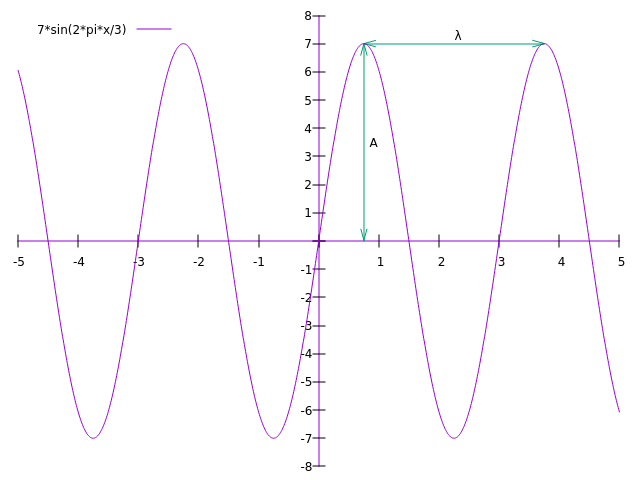
\includegraphics[width=0.6\textwidth]{sin.png}
    \caption{Elementos de una onda}
    \label{fig:elementos-onda}
\end{figure}

\subsection{Soluciones a la ecuación de onda}\label{subsec:soluciones-a-la-ecuación-de-onda}
La solución más sencilla a la ecuación de ondas es considerar una onda plana que se desplaza longitudinalmente en la dirección de la onda, donde si situamos el sistema de referencia en un punto de equilibrio tenemos la solución:
\begin{equation}
    \label{eq:solucion-ecuacion-ondas-simple}
    \psi(x,t)=A\sin(\omega t-kx)
\end{equation}

Pero la luz en una onda electro-magnética y como ya apreción Maxwell, el campo magnético aporta una componente a las ecuaciones en forma de onda compleja, y en este caso, la solución más sencilla de onda electro-magnética plana que se desplaza longitudinalmente en la dirección de la onda es:
\begin{equation}
    \label{eq:solucion-ecuacion-ondas-complejas-simple}
    \psi(x,t)=Ae^{i(\omega t-kx)}
\end{equation}

\section{Dualidad onda-partícula de De Broglie}\label{sec:dualidad-onda-partícula-de-de-broglie}

Si los fotones son partículas y ondas a la vez, podemos usar el postulado de la mecánica relativista de Einstein para partículas, y a la vez, el postulado de Planck para ondas.

\begin{postulate}[Valor de la energía de las ecuaciones de Einstein]
    \label{pos:energia_einstein}
    E=mc^2=pc
\end{postulate}

\begin{postulate}[Valor de la energía de las ecuaciones de Planck]
    \label{pos:energia_planck}
    E=h\nu=\frac{hc}{\lambda}
\end{postulate}

Así pues igualando ambas energías obtenemos la relación para cada partícula entre su momento y su longitud de onda:
\begin{postulate}[Relación entre longitud de onda y momento de De Broglie]
    \label{pos:dualidad_de_broglie}
    \lambda=\frac{h}{p}
\end{postulate}

\begin{example}
    Calcular la longitud de onda de una persona de masa $8$ kg cuando anda a una velocidad de $45$ km/h.

    La persona tiene un momento de $8*45*1000/3600=1000$ Kg m/s. Así que la longitud de onda asociada es de $\lambda=\frac{6,6256*10^{-34}}{1000}=6,6256*10^{-37}$ metros.
\end{example}

\begin{note}
    La longitud de onda más pequeña que actualmente podemos observar es del orden de $10^{-20}$ metros con el \textbf{Cherenkov telescope array}.
\end{note}

\subsection{Conclusiones}
Usando la nueva relación entre longitud de onda y momento, podemos obtener las siguientes igualdades:
\begin{equation}
    \label{eq:k_debroglie}
    k=\frac{2\pi}{\lambda}\by{\ref{pos:dualidad_de_broglie}}\frac{2\pi p}{h}=\frac{p}{\hbar}
\end{equation}
\begin{equation}
    \label{eq:omega_planck}
    \omega=2\pi\nu\by{\ref{pos:energia_planck}}2\pi\frac{E}{h}=\frac{E}{\hbar}
\end{equation}
\begin{equation}
    \label{eq:omega_debroglie}
    \omega\by{\ref{eq:omega_planck}}\frac{E}{\hbar}=\frac{p^2}{2m\hbar}\by{\ref{pos:dualidad_de_broglie}}\frac{h^2}{\lambda^2 2m\hbar}=\frac{2\pi h}{\lambda^2 2m}=\frac{\hbar k^2}{2m}
\end{equation}
\begin{equation}
    \label{eq:frecuencia_debroglie}
    \nu\by{\ref{pos:energia_planck}}\frac{E}{h}=\frac{p^2}{2mh}\by{\ref{pos:dualidad_de_broglie}}\frac{h^2}{2mh\lambda^2}=\frac{h}{2m\lambda^{2}}
\end{equation}

\subsection{Solución de onda momento-energía}\label{subsec:solucion-de-onda-momento-energia}
Una consecuencia interesante de la dualidad onda-partícula de De Blogie, es poder expresar la solución de onda electro-magnética en función de su energía y su momento.

\begin{equation}
    \label{eq:ecuacion_onda_momento_energia}
    \psi(x,t)=Ae^{i(\omega t-kx)}\by{\ref{eq:omega_planck} y \ref{eq:k_debroglie}}Ae^{i(\frac{E}{\hbar} t-\frac{p}{\hbar}x)}=Ae^{i(\hbar^{-1}(E t-p x))}
\end{equation}

\subsection{Desarrollo de la ecuación de Schröndiger}\label{subsec:desarrollo-de-la-ecuación-de-schrondiger}

Partimos de la solución de onda momento-energía (\ref{eq:ecuacion_onda_momento_energia}), calculamos la derivada parcial respecto del tiempo y la segunda derivada parcial respecto del espacio dos veces y recordando que la energia es la suma de la energía cinética y energía potencial.
\begin{equation*}
    \frac{\partial\psi}{\partial x}=\frac{ip}{\hbar}\psi\text{ y }\frac{\partial^2\psi}{\partial x^2}=\frac{-p^2}{\hbar^2}\psi
\end{equation*}

\begin{equation*}
    \frac{\partial\psi}{\partial t}=\frac{-iE}{\hbar}\psi=\frac{-ip^2}{2m\hbar}\psi+\frac{-iV}{\hbar}\psi=\frac{-i\hbar}{2m}\frac{p^2}{\hbar^2}\psi+\frac{-iV}{\hbar}\psi=\frac{i\hbar}{2m}\frac{\partial^2\psi}{\partial x^2}+\frac{-iV}{\hbar}\psi\so
\end{equation*}

\begin{equation}
    \label{eq:desarrollo-3ecuacion-schrodinger}
    i\hbar\frac{\partial\psi}{\partial t}=\frac{-\hbar^2}{2m}\frac{\partial^2\psi}{\partial x^2}+V\psi
\end{equation}



    \chapter{Ecuación de Schrödinger}

\section{Función de onda}
A la onda asociada a una partícula se le llama \define{función de onda}{funcion_de_onda} y se le suele denotar por $\Psi$.

La \define{ecuación de Schrödinger}{ecuacion_de_schrodinger}, describe la evolución temporal de la función de onda de una partícula masiva y no relativista.
\begin{postulate}[Ecuación de Schrödinger]
    \begin{equation}
    \label{eq:ecuacion_schrodinger}
    \frac{\partial\Psi(\vec{r},t)}{\partial t}=\frac{i\hbar}{2m}\nabla\Psi(\vec{r},t)-\frac{i}{\hbar}V(\vec{r},t)\Psi(\vec{r},t)
    \end{equation}
\end{postulate}

\section{Propiedades de las soluciones a la ecuación de Schrödinger}\label{sec:propiedades-de-las-soluciones-a-la-ecuación-de-schrödinger}

\subsection{Linealidad}\label{subsec:linealidad}
Es fácil comprobar que si $\Psi_1$ y $\Psi_2$ son funciones de onda para un potencial $V(x,t)$ y $a\in\C$, entonces $\Psi_1+\Psi_2$ y $a\Psi$ son ambos funciones de onda para el mismo potencial $V(x,t)$.
En cuanto a la conjugada tenemos que $\Psi^*_1$ es el opuesto a la solución de la ecuación de onda del conjudado del potencial, es decir

\begin{equation}
    \label{eq:ecuacion_schrodinger_conjugada}
    \frac{\partial\Psi^*(\vec{r},t)}{\partial t}=\frac{-i\hbar}{2m}\nabla\Psi^*(\vec{r},t)+\frac{i}{\hbar}V^*(\vec{r},t)\Psi^*(\vec{r},t)
\end{equation}

\subsubsection{Solución temporal}
Si la función de onda sólo depende del tiempo, la ecuación~\eqref{eq:ecuacion_schrodinger} queda como $\Psi^\prime(t) = -i/\hbar V(t)\Psi(t)$ cuya solución es $\Psi(t)=e^{-it(W(t)+W)/\hbar}$ donde $W^\prime (t)=V(t)$ y $W\in\C$.

\subsubsection{Solución espacial}
Si la función de onda sólo depende del espacio, la ecuación~\eqref{eq:ecuacion_schrodinger} queda como $0=-i\hbar/(2m)\nabla\Psi(\vec{r})+V(\vec{r})\Psi(\vec{r})$, es decir $\nabla\Psi(\vec{r})=-i2m/\hbar V(\vec{r})\Psi(\vec{r})$.

\subsection{Estados estacionarios}\label{subsec:estados-estacionarios}
Vamos a estudiar un caso muy especial, donde el potencial no depende del tiempo y donde la solución es el producto de una solución espacial y otra temporal, simplificaremos las ecuaciones tomando una sola variable, es decir $\Psi(x,t)=f(x)g(t)$, la ecuación~\eqref{eq:ecuacion_schrodinger} queda como $f(x)g'(t)=i\hbar/(2m)f''(x)g(t)-i/\hbar V(x)f(x)g(t)$.


\textbf{Caso 1.}

Para algún momento $t_0$ la función $g$ se anula, es decir, $f(x)g'(t_0)=0$ para todo punto del espacio, así que $g'(t_0)=0$.

\textbf{Caso 2.}

Para algún punto del espacio $x_0$ la función $f$ se anula, es decir, $0=f''(x_0)g(t)$ en todo momento, así que $f''(x_0)=0$.

\textbf{Caso 3.}

Nunca se anulan las funciones, podemos entonces dividir en todo momento la ecuación anterior por $f(x)g(t)$, quedando la ecuación $g'(t)/g(t)=i\hbar/(2m)f^{\prime\prime}(x)/f(x)-i/\hbar V(x)$.
Teniendo que una expresión temporal es igual a una expresión espacial para todo tiempo y todo espacio, esto es posible si ambas expresiones son constantes en tiempo y espacio, y deben cumplirse a la vez que para algún $C\in\C$
\begin{gather*}
    \frac{g'(t)}{g(t)}=C\Rightarrow g(t)=e^{Ct}
    \\
    \frac{i\hbar}{2m}\frac{f''(x)}{f(x)}-\frac{i}{\hbar}V(x)=C
\end{gather*}

\begin{resultado}
    Si el potencial $V$ es independiente del tiempo y $C\in\C$ cumple que $\frac{g'(t)}{g(t)}=C$, entonces $C$ es imaginario.
\end{resultado}
\begin{proof}
    Si calculamos la norma al cuadrado de $\Psi$ tenemos que
    \begin{equation*}
        \nor{\Psi(x,t)}^2=\Psi^*(x,t)\Psi(x,t)=f^*(x)g^*(t)f(x)g(t)=\nor{f(x)}^2\nor{g(t)}^2
    \end{equation*}
    Usando la ecuación~\eqref{eq:ecuacion_probabilidad_onda} tenemos que
    \begin{equation*}
        1=\int_{-\infty}^{+\infty}\nor{\Psi(x,t)}^2 dx=\nor{g(t)}^2\int_{-\infty}^{+\infty}\nor{f(x)}^2 dx
    \end{equation*}
    Para que la ecuación anterior sea cierta, la norma de $g$ debe ser una constante, es decir, $g^*(t)g(t)=e^{C^*t}e^{Ct}=e^{(C^*+C)t}$ debe ser constante en el tiempo, por tanto se tiene como única opción que $C^*+C=0$, es decir, que $C$ sea un número imaginario.
\end{proof}

\begin{resultado}
    Si el potencial $V$ es independiente del tiempo y $\Psi(x,t)=f(x)g(t)$ se cumple que $\nor{\Psi(x,t)}^2=\nor{f(x)}^2$.
\end{resultado}
\begin{proof}
    Como hemos visto en el resultado anterior, $\nor{g(t)}^2=1$, y por tanto
    \begin{equation}
        \label{eq:probabilidad_atemporal}
        \nor{\Psi(x,t)}^2=\nor{f(x)}^2\nor{g(t)}^2=\nor{f(x)}^2
    \end{equation}
\end{proof}
Así que $C=iD$ con $D\in\R$, las soluciones al estado estacionario queda como
\begin{gather*}
    \frac{g'(t)}{g(t)}=iD
    \\
    \frac{\hbar}{2m}\frac{f''(x)}{f(x)}-\frac{1}{\hbar}V(x)=D
\end{gather*}

\subsubsection{Hamiltoniano}
Si consideramos el conjunto de la energía cinética más la energía potencial, obtenemos lo que llamamos el \define{Hamiltoniano} y tiene la expresión
\begin{equation}
    \label{eq:halmitoniano}
    H(x,p)=\frac{p^2}{2m}+V(x)
\end{equation}
Llamamos \define{operador Hamiltoniano} al operador definido por
\begin{equation}
    \label{eq:operador_hamiltoniano}
    \widehat{H}=-\frac{\hbar^2}{2m}\frac{\partial^2}{\partial x^2}+V(x)
\end{equation}
Usando el operador Hamiltoniano en la ecuación~\eqref{eq:ecuacion_schrodinger_tempoespacial} podemos expresarlo así
\begin{equation*}
    \widehat{H}f(x)=-i\hbar Df(x)
\end{equation*}
Para simplificar la expresión llamamos $E=-\hbar D$ y por tanto las soluciones al estado estacionario queda como
\begin{gather*}
    \frac{g'(t)}{g(t)}=-iE/\hbar
    \\
    \frac{\hbar}{2m}\frac{f''(x)}{f(x)}-\frac{1}{\hbar}V(x)=-E/\hbar\Rightarrow \frac{\hbar^2}{2m}\frac{f''(x)}{f(x)}-V(x)=-E
\end{gather*}

\begin{definicion}
    Llamamos \define{Ecuación de Schrödinger independiente del tiempo} a la ecuación solución de la parte espacial del estado estacionario
    \begin{equation}
        \label{eq:ecuacion_schrodinger_tempoespacial}
        -\frac{\hbar^2}{2m}f''(x)+V(x)f(x)= Ef(x)
    \end{equation}
\end{definicion}

Resolviendo la ecuación diferencial temporal y usando el operador de Halmiton podemos dejar las soluciones de estados estacionarios como
\begin{equation}
    \label{eq:solucion_estado_estacionario}
    \Psi(x,t)=f(x)g(t)\text{ donde }
    \begin{cases}
        g(t)=e^{-iEt/\hbar}\\
        \widehat{H}f(x)=Ef(x)\\
        E\in\R
    \end{cases}
\end{equation}

\subsection{Observaciones a las soluciones del estado estacionario}\label{subsec:observaciones-a-las-soluciones-del-estado-estacionario}

\subsubsection{Solución general}
La solución general del estado estacionario se puede expresar como
\begin{equation}
    \label{eq:solucion_general_estado_estacionario}
    \Psi(x,t)=\sum_{k\in\N}c_k f_k(x)e^{-iE_k t/\hbar}
\end{equation}
Donde $\forall k\in\N$ $E_k\in\R$ y $\widehat{H}f_k(x)=E_k f_k(x)$

\subsubsection{Desviación de H}
$\avg{H} = \int_{-\infty}^{+\infty}\Psi^* \widehat{H}\Psi dx = \int_{-\infty}^{+\infty}\Psi^* E\Psi dx=E\int_{-\infty}^{+\infty}\Psi^* \Psi dx = E$

$\avg{H^2} = \int_{-\infty}^{+\infty}\Psi^* \widehat{H}^2\Psi dx = \int_{-\infty}^{+\infty}\Psi^* E^2\Psi dx=E^2\int_{-\infty}^{+\infty}\Psi^* \Psi dx = E^2$

Por tanto $\sigma_H=\avg{H^2}-\avg{H}^2=E^2-E^2=0$

    \chapter{Probabilidad cuántica}\label{ch:probabilidad-cuántica}

Una vez vista las propiedades de la función de onda de una partícula, y estudiado algunos casos, volvemos a preguntarnos sobre la partícula, ¿que información podemos obtener si conocemos su función de onda?.
La relación entre la partícula y su función de onda, es probabilística, y exactamente tenemos que $\abs{\fuconda(\vec{r}, t)}^2 d^3\vec{r}$ representa la probabilidad de encontrar a la partícula en el mommento $t$ en el punto $\vec{r}$.

Como la partícula debe estar en algún punto del espacio, se tiene que cumplir
\begin{postulate}[Condición probabilística de la ecuación de ondas]
    \begin{equation}
        \label{eq:condicion_probabilistica_fuconda}
        \int_{\R^3}\abs{\fuconda(\vec{r}, t)}^2 d^3\vec{r}=1
    \end{equation}
\end{postulate}

\subsection{Espacio de Hilbert}\label{subsec:espacio-de-hilbert}

Como vimos en~\ref{sec:propiedades-de-las-soluciones-a-la-ecuación-de-schrödinger}, las combinaciones lineales de soluciones de la ecuación de Schrödinger, son también soluciones, por tanto el conjunto de las soluciones a la ecuación de Schrödinger es un subespacio de las funciones de cuadrado integable $\mathscr{L}^2$ que es un espacio de Hilbert.
    %\chapter{Espacios de Hilbert}

\section{Notación Cuántica}
A partir de este punto, vamos a usar la notación cuántica de Dirac:
\begin{itemize}
  \item Denotaremos por $\mathbb{H}$ a los espacios de Hilbert y a sus vectores por $\ket{x}$.
  \item Llamamos operadores a los homomorfismos entre espacios de Hilbert y los denotamos por $\hat{f}$.
  \item Denotaremos a la función dual de $\ket{x}$ por $\bra{x}$.
  \item Denotaremos al producto escalar de $\ket{x}$ y $\ket{y}$ por $\braket{x}{y}$.
  \item Denotaremos la expresión $\operatoravg{x}{\hat{f}}{y}$ al producto escalar de ${\ket{x}}$ y $\ket{\hat{f}(y)}$.
\end{itemize}

Mientras no se indique lo contrario, siempre un espacio vectorial será un $\C$-espacio vectorial.

\subsection{Espacios métricos}
\begin{definition}
  \label{distancia}
  Sea $E$ un espacio vectorial, diremos que la aplicación $d:E \rightarrow \R$ es una \define{métrica}{métrica} sobre $E$ si cumple:
  \begin{itemize}
    \item $\forall x,y \in E,\ d(x,y)=d(y,x)$.
    \item $\forall x,y,z \in E,\ d(x,z)\leq d(x, y)+d(y, z)$.
    \item $\forall x, y \in E,\ d(x,y)\geq 0 \text{ siendo } d(x,y)=0\Leftrightarrow x = y$.
  \end{itemize}
\end{definition}

\begin{definition}
  \label{espacio_metrico}
  Sea $E$ un espacio vectorial y $d$ una métrica sobre $E$, llamamos al par $(E, d)$ un \define{espacio métrico}.
\end{definition}

\subsection{Espacios normados}
\begin{definition}
  \label{norma}
  Sea $E$ un espacio vectorial, diremos que la aplicación $\nor{}:E \rightarrow \R$ es una \define{norma} sobre E si cumple:
  \begin{itemize}
    \item $\forall x \in E,\ \forall\alpha\in\C,\ \nor{\alpha x}=\abs{\alpha}\nor{x}$.
    \item $\forall x,y \in E,\ \nor{x+y}\leq\nor{x}+\nor{y}$.
    \item $\forall x \in E,\ \nor{x}\geq 0 \text{ siendo } \nor{x}=0\Leftrightarrow x = 0$.
  \end{itemize}
\end{definition}

\begin{definition}
  \label{espacio_normado}
  Sea $E$ un espacio vectorial y $\nor{}$ una norma sobre $E$, llamamos al par $(E, \nor{})$ un \define{espacio normado}.
\end{definition}

Todo espacio normado $(E, \nor{})$, es un espacio métrico, definiendo la métrica para cada par de elementos, $x, y\in E$ por $d(x, y)=\nor{x-y}$. Esta métrica se denomina \define{métrica definida por la norma}.

\definicion{Sean $(E, \nor{})$ y $(E', \nor{}')$ dos espacios normados. Sea f un homomorfismo entre E y E'. Diremos que \define{f es acotado} si existe
$c\in\R^+$ tal que $\nor{f(x)}' \leq c\nor{x}\ \forall x\in E$. Diremos que c es una \define{cota de f}.}

\definicion{Sea f un homomorfismo acotado sobre dos espacios normados. Llamamos \define{norma de f} al ínfimo de las
cotas de f.}

\resultado{
Un homomorfismo sobre espacios normados es continuo si y sólo si es acotado.
}

\resultado{
Un homomorfismo sobre espacios normados es continuo si y sólo si es continuo en un elemento.
}

\ejercicio{
Sean $E$ y $F$ dos espacios normados y $C$ el espacio vectorial de los homomorfismo acotados de $E$ en $F$. Demostrar que $\forall\ T\in C$ definiendo $\nor{T}=\text{sup}_{x\in E-\{0\}}\frac{\nor{T(x)}}{\nor{x}}$ es una norma en $C$.
}

\subsection{Espacios Euclídeos}
\begin{definition}
  \label{producto_escalar}
  Sea $E$ un espacio vectorial, diremos que la aplicación $\braket{}{}:E\times E \rightarrow \C$ es un \define{producto escalar} sobre E si cumple:
  \begin{itemize}
    \item $\forall x,y \in E,\ \braket{x}{y}=\overline{\braket{y}{x}}$.
    \item $\forall x,y,z \in E, \braket{x}{y+z}=\braket{x}{y}+\braket{x}{z}$.
    \item $\forall x,y \in E,\ \forall\alpha\in\C, \braket{x}{\alpha y}=\overline{\alpha}\braket{x}{y}$.
    \item $\forall x \in E, \braket{x}{x}\geq 0 \text{ siendo } \braket{x}{x}=0\Leftrightarrow x = 0$.
  \end{itemize}
\end{definition}

\begin{definition}
  \label{espacio_euclideo}
  Sea $E$ un espacio vectorial y $\braket{}{}$ un producto escalar sobre $E$, llamamos al par $(E, \braket{}{})$ un \define{espacio euclídeo}.
\end{definition}

Todo espacio euclídeo $(E, \braket{}{})$, es un espacio normado, definiendo la norma para cada $x\in E$, por $\nor{x}=\sqrt{\braket{x}{x}}$. Esta norma se denomina \define{norma definida por el producto escalar}.

En realidad, no es necesario indicar cual es la métrica, la norma o el producto escalar usado, pues siempre sabemos cada elemento a que espacio pertenece, así pues, sólo diremos que $E$ es un espacio métrico, euclídeo o normado y siempre denotaremos por $d$ la métrica, por $\nor{}$ la norma y por $\braket{}{}$ el producto escalar.

\begin{proposition}[Riesz]
  Sean $E$ y $F$ dos espacios euclídeos y $C$ el espacio normado de los homomorfismos acotados entre $E$ y $F$. Para cada $f\in C$, existe $z_f\in E$ tal que para todo $x\in\ E$ se tiene que $f(x)=\braket{x}{z_f}$ y además $\nor{z_f}=\nor{f}$.
\end{proposition}

\begin{definition}
  Sea $(E, \braket{}{})$ un espacio euclídeo, con $X=\{x_n\}_{n\in\N}$ un conjunto de vectores linealmente independintes. Si $x\in E$, llamamos \define{serie de Fourier de $x$ con respecto a $X$} a
  \begin{equation}
    \sum_{n\in\N}\braket{x}{x_n}x_n
  \end{equation}
\end{definition}

\begin{proposition}
  \label{norma_suma_general}
  Sea E un espacio euclídeo, dados $f,g\in E$ y $a,b\in\C$, se tiene la siguiente igualdad:
  \begin{equation}
    \nor{af+bg}^2=\abs{a}^2\nor{f}^2+\abs{b}^2\nor{g}^2+2\Re(a\overline{b}\braket{f}{g})
  \end{equation}
\end{proposition}
\begin{proof}
  \nor{af+bg}^2=\braket{af+bg}{af+bg}=\braket{af}{af}+\braket{af}{bg}+\braket{bg}{af}+\braket{bg}{bg}=\abs{a}^2\nor{f}^2+a\overline{b}\braket{f}{g}+b\overline{a}\braket{g}{f}+\abs{b}^2\nor{g}^2=\abs{a}^2\nor{f}^2+\abs{b}^2\nor{g}^2+a\overline{b}\braket{f}{g}+\overline{a\overline{b}}\overline{\braket{f}{g}}=\abs{a}^2\nor{f}^2+\abs{b}^2\nor{g}^2+a\overline{b}\braket{f}{g}+\overline{a\overline{b}\braket{f}{g}}=\abs{a}^2\nor{f}^2+\abs{b}^2\nor{g}^2+2\Re(a\overline{b}\braket{f}{g}).
\end{proof}
\begin{proposition}
  \label{producto_escalar_real}
  Sea E un espacio euclídeo, dados $f,g\in E$ se tiene la siguiente desigualdad:
  \begin{equation}
    \Re(\braket{f}{g})\leq\frac{1}{2}(\nor{f}^2+\nor{g}^2)
  \end{equation}
\end{proposition}
\begin{proof}
  Usando el resultado~\eqref{norma_suma_general} para $a=1$ y $b=-1$ tenemos que $\abs{a}=1$, $\abs{b}=1$ y $a\overline{b}=-1$ y la igualdad queda
  \begin{equation*}
    \nor{f-g}^2=\nor{f}^2+\nor{g}^2+2\Re(-\braket{f}{g})
  \end{equation*}
  Como la norma de cualquier vector es mayor o igual que cero, tendremos que
  $0\leq\nor{f}^2+\nor{g}^2+2\Re(-\braket{f}{g})=\nor{f}^2+\nor{g}^2-2\Re(\braket{f}{g})\Rightarrow 2\Re(\braket{f}{g})\leq\nor{f}^2+\nor{g}^2\Rightarrow \Re(\braket{f}{g})\leq\frac{1}{2}(\nor{f}^2+\nor{g}^2)$.
\end{proof}

\begin{proposition}
  \label{exponencial_producto_interno_real}
  Sea E un espacio euclídeo, dados $f,g\in E$ se tiene la siguiente igualdad:
  \begin{equation}
    max\{\Re(e^{i\alpha}\braket{f}{g})\text{ tq }\alpha\in\C\}=\abs{\braket{f}{g}}
  \end{equation}
\end{proposition}
\begin{proof}
  Tenemos que $\braket{f}{g}=a+ib$ para algún $a,b\in\R$. Así que $e^{i\alpha}\braket{f}{g}=(\cos(\alpha)+i \sin(\alpha))(a+ib)=(a \cos(\alpha)-b \sin(\alpha)) + i(b \cos(\alpha)+a\sin(\alpha)).$

  Por tanto, la parte real es $\Re(e^{i\alpha}\braket{f}{g})=a \cos(\alpha)-b \sin(\alpha)$ para todo $\alpha\in\C$, por lo tanto la parte real está incluido en la circunferencia de radio $\sqrt{a^2+b^2}$ y el máximo de estos valores se alcanza precisamente en la frontera del círculo, es decir $\sqrt{a^2+b^2}$ que es $\abs{\braket{f}{g}}$.
\end{proof}
\begin{proposition}
  \label{norma_producto_escalar_producto_norma}
  Sea E un espacio euclídeo, dados $f,g\in E$ se tiene la siguiente desigualdad:
  \begin{equation}
    \abs{\braket{f}{g}}\leq\nor{f}\nor{g}
  \end{equation}
\end{proposition}

\begin{proof}
  Usando el resultado~\eqref{norma_suma_general} y fijando $\alpha\in\C$, para $a=\frac{\nor{g}}{\nor{f}}e^{i\alpha}$ y $b=-\frac{\nor{f}}{\nor{g}}$ tenemos que $\abs{a}=\frac{\nor{g}}{\nor{f}}$, $\abs{b}=\frac{\nor{f}}{\nor{g}}$ y $a\overline{b}=-e^{i\alpha}$ y la igualdad queda
  \begin{multline*}
    \nor{\frac{\nor{g}}{\nor{f}}e^{i\alpha}f-\frac{\nor{f}}{\nor{g}}g}^2=\frac{\nor{g}}{\nor{f}}\nor{f}^2+\frac{\nor{f}}{\nor{g}}\nor{g}^2+2\Re(-e^{i\alpha}\braket{f}{g})=\\
    =\nor{g}\nor{f}+\nor{f}\nor{g}-2\Re(e^{i\alpha}\braket{f}{g})=2(\nor{f}\nor{g}-\Re(e^{i\alpha}\braket{f}{g}))
  \end{multline*}
  Como la norma de cualquier vector es mayor o igual que cero, tenemos que
  $0\leq\nor{f}\nor{g}-\Re(e^{i\alpha}\braket{f}{g})\Rightarrow \Re(e^{i\alpha}\braket{f}{g})\leq\nor{f}\nor{g}$.

  Como la desigualdad anterior es válida para todo $\alpha\in\C$ y usando el resultado~\eqref{exponencial_producto_interno_real} tendremos que $ \abs{\braket{f}{g}}\leq\nor{f}\nor{g}$.
\end{proof}

\begin{proposition}
  Sea E un espacio euclídeo, dados $f,g\in E$ se tiene que:
  \begin{equation}
    \label{norma_producto_escalar_igual_producto_norma}
    \abs{\braket{f}{g}}=\nor{f}\nor{g}\Leftrightarrow \exists\alpha\in\C\text{ tq }f=\alpha g
  \end{equation}
\end{proposition}

\begin{proof}
  Primero vamos a considerar el caso $f=\alpha g$:
  \begin{equation*}
    \abs{\braket{f}{g}}=\abs{\braket{\alpha g}{g}}=\abs{\alpha}\nor{g}^2=\abs{\alpha}\nor{g}\nor{g}=\nor{f}\nor{g}
  \end{equation*}
  Para el caso contrario, como se comprobó en el resultado~\eqref{norma_producto_escalar_producto_norma}, $\braket{f}{g}$ es el valor máximo de $\Re(e^{i\alpha}\braket{f}{g})$. Como dichos valores forman un conjunto cerrado, el máximo se alcanza, es decir, existe $\beta\in\C$ tal que $\Re(e^{i\beta}\braket{f}{g})=\abs{\braket{f}{g}}$ y utilizando el resultado~\eqref{norma_suma_general} para $a=\frac{\nor{g}}{\nor{f}}e^{i\beta}$ y $b=-\frac{\nor{f}}{\nor{g}}$ tenemos que:
  \begin{multline*}
    \nor{\frac{\nor{g}}{\nor{f}}e^{i\beta}f-\frac{\nor{f}}{\nor{g}}g}=2(\nor{f}\nor{g}-\Re(e^{i\beta}\braket{f}{g}))=2(\nor{f}\nor{g}-\braket{f}{g})=\\
    =2(\nor{f}\nor{g}-\nor{f}\nor{g})=0
  \end{multline*}
  Si la norma es igual que cero, tenemos que
  $\frac{\nor{g}}{\nor{f}}e^{i\beta}f=\frac{\nor{f}}{\nor{g}}g\Rightarrow f=e^{-i\beta}\frac{\nor{f}^2}{\nor{g}^2}g$. Y por tanto para $\alpha=e^{-i\beta}\frac{\nor{f}^2}{\nor{g}^2}$ tenemos la igualdad buscada.
\end{proof}

\subsection{Espacios de Banach}
\begin{definition}
  \label{espacio_banach}
  Un espacio normado es un \define{espacio de Banach} si es completo para la métrica definida por la norma.
\end{definition}

\subsection{Espacios de Hilbert}
\begin{definition}
  \label{espacio_hilbert}
  Un espacio euclídeo es un \define{espacio de Hilbert} si es completo para la norma inducida.
\end{definition}

\resultado[Ortogonalización de Gram-Schmidt]{
Todo subespacio vectorial de un espacio de Hilbert admite una base ortonormal.
}
\resultado{
Sean $E$ y $F$ dos espacios de Hilbert. Para todo homomorfismo $f$ de $E$ a $F$ existe un homomorfismo $f^+$ de $F$ a $E$ tal que $\braket{f(x)}{y}=\braket{x}{f^+(y)}$.
}

\begin{definition}
  \label{homomorfismo_adjunto}
  Sean $E$ y $F$ dos espacios de Hilbert y $f$ un homomorfismo de $E$ a $F$. Llamamos \define{homomorfismo adjunto de f} al homomorfismo $f^+$ de $F$ a $E$ tal que $\braket{f(x)}{y}=\braket{x}{f^+(y)}$.
\end{definition}

\resultado{
Sean $f$ y $g$ homomorfismos entre espacios de Hilbert. Se cumple:
\begin{itemize}
  \item $(f^+)^+=f$.
  \item $(af)^+=\overline{a}f^+$ para todo $a\in\C$.
  \item $(fg)^+=g^+f^+$.
\end{itemize}
}

\resultado{
Sean $f$ y $g$ dos homomorfismos entre espacios de Hilbert. El producto $fg$ es hermítico si y sólo si $f$ y $g$ conmutan.
}

\definicion{
Sean $f$ y $g$ dos homomorfismos entre espacios de Hilbert. Llamamos \define{conmutador de f}
}

\resultado{
Sean $f$ y $g$ dos homomorfismos entre espacios de Hilbert.
}

\begin{definition}
  \label{automorfismo_autoadjunto}\label{automorfismo_hermitico}
  Sean $E$ un espacio de Hilbert y $f$ un automorfismo de $E$. Diremos que \define{f es autoadjunto} o \define{hermítico} si $f = f^+$.
\end{definition}

\begin{definition}
  Sean $E$ y $F$ dos espacios de Hilbert y $f$ un homomorfismo de $E$ a $F$. Diremos que \define{$f$ es compacto} si para toda sucesión $(x_n)_{n\in\N}$ de $E$, la sucesión $(f(x_n))_{n\in\N}$ tiene una subsucesión convergente.
\end{definition}

\resultado{
Todo automorfismo compacto y hermítico sobre un espacio de Hilbert tiene su norma o el opuesto de su norma como valor própio.
}

\resultado[Teorema espectral]{
Sea $E$ un espacio de Hilbert y $f$ un automorfismo hermítico y compacto. El conjunto de todos los autovectores ortonormales de $f$ es numerable.
}

\subsection{Espacios de Hilbert separable}
\begin{definition}
  \label{espacio_hilbert_separable}
  Un espacio de Hilbert es un \define{espacio de Hilbert separable} si tiene un subconjunto denso numerable.
\end{definition}

\resultado{
Sea $E$ un espacio de Hilbert separable y $f$ un automorfismo de $E$. Si $f$ tiene un número infinito de valores propios distintos, entonces es una cantidad numerable y ordenados de mayor a menor definen una sucesión convergente a 0.
}

\resultado{
Sea $E$ un espacio de Hilbert separable y $f$ un automorfismo hermítico y compacto. El conjunto $\{e_n\}_{n\in\N}$ de todos los vectores propios ortonormales de $f$ es una base de $E$. Ademas se tiene que para todo $x\in\ E$, $f(x)=\sum_{n\in\N}\lambda_n\braket{x}{e_n}e_n$, donde $\lambda_n$ es el valor propio asociado al vector propio $e_n$.
}

\resultado{
En un espacio de Hilbert separable, todos los conjuntos ortogonales son numerables.
}

    %\chapter{2}\label{ch:2}
\section{Matrices}

Mientras no se indique lo contrario, las matrices son cuadradas, de dimensión $n$ y sobre el cuerpo de los números complejos.

Si $\mathbf{A}$ es una matriz, llamamos a sus elementos $\mathbf{A}_i^j$. A la $i$-ésima fila de $\mathbf{A}$ la denotamos por $\mathbf{A}_i$ y a la $i$-ésima columna de $\mathbf{A}$ la denotamos por $\mathbf{A}^i$.

Dada una matriz $\mathbf{A}=(\mathbf{A}_i^j)$ podemos definir los siguientes conceptos:
\begin{tabular}{l|l|l}
	Mombre & Notación & Definición \\
	\hline
	Matriz adjunta & $\mathbf{A}^T$ & ${\mathbf{A}^T}_i^j := \mathbf{A}_j^i$. \\
	Diagonal & $\text{diag}(\mathbf{A})$ & $(\mathbf{A}_1^1, \dots, \mathbf{A}_n^n)$. \\
	& $\mathbf{A}|_i^j$ & $\mathbf{A}$ quitando la $i$-ésima fila y la $j$-ésima columna. \\
	menor de $\mathbf{A}_i^j$ & & det$(\mathbf{A}|_i^j)$. \\
	cofactor de $\mathbf{A}_i^j$ & $\mathbf{\tilde{A}}_i^j$ & $(-1)^{i+j}$ det$(\mathbf{A}|_i^j)$. \\
	adjunto & adj$(\mathbf{A})$ & $(\text{adj}(\mathbf{A}))_i^j := \mathbf{\tilde{A}}_i^j$. \\
	$\mathbf{A}$ es ortogonal & & Si $\mathbf{A}\mathbf{A}^T=\mathbf{A}^T\mathbf{A}=\mathbf{I}$.
\end{tabular}

\paragraph{Resultados}
\begin{itemize}
	\item Sea $\mathbf{A}$ una matriz, $\mathbf{A}\text{adj}(\mathbf{A}) = \text{adj}(\mathbf{A})\mathbf{A}=\text{det}(\mathbf{A})\mathbf{I}$.
	\item Sea $\mathbf{A}$ una matriz ortogonal, entonces det$(\mathbf{A})=\pm1$.
\end{itemize}


    %\chapter{4}\label{ch:4}
\section{Definiciones y notación}
\begin{definicion}
    Sea $I$ un intervalo abierto de $\R$. Llamamos \define{Espacio cuántico de $I$} a
    \begin{equation}
        EC_I=\{f:\R\rightarrow\C\mid\int_I\nor{f(x)}^2 dx \in \R\}
    \end{equation}
\end{definicion}

El espacio cuántico es un espacio vectorial de dimensión infinita y en el cual tenemos definido el producto interno
\begin{equation}
    \forall f,g\in EC_I \ \langle f,g \rangle=\int_I f^* g\ dx
\end{equation}

\begin{definicion}
    Diremos que un vector está \define{normalizado} si su norma es 1.
\end{definicion}

Las funciones de onda (vectores) reciben el nombre de \textbf{ket} y se denota por $\ket{f}$, los operadores (funciones lineales) reciben el nombre de \textbf{bra} y se denota por $\bra{H}$. Llamamos \define{braket} y se denota por $\braket{f}{g}$ al producto interno y por $\operatoravg{f}{H}{g}$ al producto interno de $f$ por $H(g)$.

\begin{definicion}
    Sea $I$ un intervalo abierto de $\R$ y $f$ un elemento de $EC_I$ y $H$ un operador sobre $EC_I$. Llamamos \define{Valor esperado de $f$ al operarlo $H$} a
    \begin{equation}
        \avg{H(f)}=\operatoravg{f}{H}{f}
    \end{equation}
\end{definicion}


\begin{definicion}
    Sea $I$ un intervalo abierto de $\R$ y $H$ un operador sobre $EC_I$. Diremos que $H$ es \define{hermitiano} si
    \begin{equation}
        \braket{f}{H(f)}=\braket{H(f)}{f}\forall f\in EC_I
    \end{equation}
\end{definicion}

    %\chapter{6}\label{ch:6}
\section{Operadores especiales}
\subsection{Operador posición}
\definicion{
Sea $f$ un automorfismo sobre el espacio de Hilbert $\L(\R^2)$. Definimos el \define{operador posición} por $\hat{X}$ actuando como $\hat{X}(f(x))=xf(x)$.
}

\resultado{
El operador posición es hermítico.
}

\subsection{Operador momento lineal}
\definicion{
Sea $f$ un automorfismo sobre el espacio de Hilbert $\L(\R^2)$. Definimos el \define{operador momemto lienal} por $\hat{P}$ actuando como $\hat{P}(f(x))=-ih\frac{df(x)}{dx}$.
}

\resultado{
El operador momento lineal es hermítico.
}

\subsection{Operador espejo}
\definicion{
Sea $f$ un automorfismo sobre el espacio de Hilbert $\L(\R^2)$. Definimos el \define{operador espejo} por $\hat{E}$ actuando como $\hat{E}(f(x))=f(-x)$.
}

\resultado{
El operador espejo es hermítico.
}

    \chapter{Resultados básicos en Análisis}\label{ch:resultados_basicos_analisis}


\section{Polinomio de Taylor}\label{sec:polinomio-de-taylor}

\subsection{Taylor en una variable}\label{subsec:taylor_una_variable}
Sea $f$ una función real definido en un intervalo abierto y $x_0$ un número del dominio, existe $\epsilon>0\in\R$ tal que $\forall\ x\in(x_0-\epsilon\coma x_0+\epsilon)$ se tiene que
\begin{equation}
    \label{eq:polinomio-taylor}
    f(x)=\sum_{n=0}^{\infty} \frac{f^{(n)}(x_0)}{n !}(x-x_0)^n
\end{equation}

\subsection{Taylor en dos variables}\label{subsec:taylor_dos_variables}
Sea $f$ una aplicación de $\R^2$ en $\R^2$, definido en un intervalo abierto y $(x_0, y_0)$ un elemento del dominio, existe $\epsilon > 0 \in\R$ tal que $\forall\ (x, y)\in(x_0-\epsilon\coma x_0+\epsilon)\times(y_0-\epsilon, y_0+\epsilon)$ se tiene que
\begin{equation}
    \label{eq:polinomio-taylor-dos-variables}
    f(x,y)=\sum_{n=0}^{\infty} \sum_{m=0}^{\infty} \frac{\partial^{n+m}f(x_0, y_0)}{\partial^n x\partial^m y}\frac{(x-x_0)^n(y-y_0)^m}{n!m!}
\end{equation}


\section{Diferencial de un funcional}\label{sec:diferencial_funcional}
Sean $E, F$ dos espacios vectoriales normados, $a\in E$ y $f$ una aplicación en un entorno $U$ de $a$ en $F$. Diremos que $f$ es diferenciable en $a$ si existe una aplicación lineal y continua $\maps{u}{E}{F}$ y una función $\rho$ definida en algún entorno del $0\in E$ con valores en $F$ tal que
\begin{subequations}
    \begin{equation*}
        lim_{x\to\infty}\rho(x)=0
    \end{equation*}
    \begin{equation*}
        f(x+h)-f(x)=u(h)+\nor{h}\rho(h)
    \end{equation*}
\end{subequations}


    \chapter{Formulario}\label{ch:formulario}
En este capítulo vamos a recoger todas las ecuaciones, fórmulas, resultados que hemos usado de forma habitual.

\section{Ecuaciones diferenciables}\label{sec:ecuaciones-diferenciables}
\subsection{Polinomio de segundo grado}\label{subsec:polinomio-de-segundo-grado}
La solución a la ecuación polinómica de segundo grado $ay^{''}+by^{'}+c=0$, se basa en calcular las raices $r_1\coma r_2$ del polinomio
$ax^2+bx+c$
\begin{itemize}
    \item Si $r_1\neq r_2\in\R\so y(x)=c_{1}e^{r_{1}x}+c_{2}e^{r_{2}x}$.
    \item Si $r_1= r_2\in\R\so y(x)=(c_{1}+c_{2}x)e^{r_{1}x}$.
    \item Si $r_1= \overline{r_2}=\alpha+i\beta\in\C\so y(x)=(c_{1}\cos(\beta x)+c_{2}\sin(\beta x))e^{\alpha x}$.
\end{itemize}

\section{Integrales}\label{sec:integrales}
\subsection{Integral de Gauss}\label{subsec:integral-de-gauss}
\subsubsection*{Integral de Gauss simple}
\begin{equation}
    \label{eq:integral-gauss}
    \int_{-\infty}^{+\infty} e^{-x^{2}}dx =\sqrt{\pi}
\end{equation}

\subsubsection*{Integral de Gauss generalizada}
\begin{equation}
    \label{eq:integral-gauss-generalizada}
    \int_{-\infty}^{+\infty} ae^{-(x+b)^{2}/c^2}dx =a\abs{c}\sqrt{\pi}
\end{equation}

\subsubsection*{Integral de Gauss con potencias pares}
\begin{equation}
    \label{eq:integral-gauss-generalizada-potencias-pares}
    \int_{-\infty}^{+\infty} x^{2n}e^{-\frac{1}{2}ax^{2}}dx =\left(\frac{2\pi}{a}\right)^{\frac{1}{2}}\frac{1}{a^n}(2n-1)!!
\end{equation}


    %\chapter{ElegantBook Settings}

This template is based on the Standard \LaTeX{} book class, so the options of book class work as well (Note that the option of papersize has no effect due to \lstinline{device} option). The default encoding is UTF-8 while \TeX{} Live is recommended. The test environment is Win10 + \TeX{} Live 2021, either \hologo{pdfLaTeX} or \hologo{XeLaTeX} works fine. \hologo{XeLaTeX} is preferred for Chinese articles.


\section{Color Themes}
This template contains 5 color themes, i.e. \textcolor{structure1}{\lstinline{green}}\footnote{Original default theme.}, \textcolor{structure2}{\lstinline{cyan}}, \textcolor{structure3}{\lstinline{blue}}(default), \textcolor{structure4}{\lstinline{gray}}, \textcolor{structure5}{\lstinline{black}}. You can choose \lstinline{green} with
\begin{lstlisting}
\documentclass[green]{elegantbook} %or
\documentclass[color=green]{elegantbook}
\end{lstlisting}


\begin{table}[htbp]
    \caption{ElegantBook Themes\label{tab:color thm}}
    \centering
    \begin{tabular}{ccccccc}
        \toprule
        & \textcolor{structure1}{green}
        & \textcolor{structure2}{cyan}
        & \textcolor{structure3}{blue}
        & \textcolor{structure4}{gray}
        & \textcolor{structure5}{black}
        & Main Environments\\
        \midrule
        structure & \makecell{{\color{structure1}\rule{1cm}{1cm}}}
        & \makecell{{\color{structure2}\rule{1cm}{1cm}}}
        & \makecell{{\color{structure3}\rule{1cm}{1cm}}}
        & \makecell{{\color{structure4}\rule{1cm}{1cm}}}
        & \makecell{{\color{structure5}\rule{1cm}{1cm}}}
        & chapter section subsection \\
        main & \makecell{{\color{main1}\rule{1cm}{1cm}}}
        & \makecell{{\color{main2}\rule{1cm}{1cm}}}
        & \makecell{{\color{main3}\rule{1cm}{1cm}}}
        & \makecell{{\color{main4}\rule{1cm}{1cm}}}
        & \makecell{{\color{main5}\rule{1cm}{1cm}}}
        & definition exercise problem  \\
        second & \makecell{{\color{second1}\rule{1cm}{1cm}}}
        & \makecell{{\color{second2}\rule{1cm}{1cm}}}
        & \makecell{{\color{second3}\rule{1cm}{1cm}}}
        & \makecell{{\color{second4}\rule{1cm}{1cm}}}
        & \makecell{{\color{second5}\rule{1cm}{1cm}}}
        & theorem lemma corollary\\
        third & \makecell{{\color{third1}\rule{1cm}{1cm}}}
        & \makecell{{\color{third2}\rule{1cm}{1cm}}}
        & \makecell{{\color{third3}\rule{1cm}{1cm}}}
        & \makecell{{\color{third4}\rule{1cm}{1cm}}}
        & \makecell{{\color{third5}\rule{1cm}{1cm}}}
        & proposition\\
        \bottomrule
    \end{tabular}
\end{table}

If you want to customize the colors, please select \lstinline{nocolor} or use \lstinline{color=none} and declare the main, second, and third colors in the preamble section as follows:
\begin{lstlisting}[frame=single]
\definecolor{structurecolor}{RGB}{60,113,183}
\definecolor{main}{RGB}{0,166,82}%
\definecolor{second}{RGB}{255,134,24}%
\definecolor{third}{RGB}{0,174,247}%
\end{lstlisting}


\section{Cover}

\subsection{Customized Cover}
Customized cover is allowed, you can choose or hide any element as you prefer. Current optional elements are:
\begin{itemize}
    \item title: \lstinline{\title}
    \item subtitle: \lstinline{\subtitle}
    \item author: \lstinline{\author}
    \item institute: \lstinline{\institute}
    \item date: \lstinline{\date}
    \item version: \lstinline{\version}
    \item extra information: \lstinline{\extrainfo}
    \item cover image: \lstinline{\cover}
    \item logo: \lstinline{\logo}
\end{itemize}

Besides, an extra command \lstinline{\bioinfo} is provided with two options--caption and content. For instance, if you want to display \lstinline{Username: 111520}, just type in

\begin{lstlisting}
\bioinfo{Username}{115520}
\end{lstlisting}

You can change the color of the horizontal bar of the cover by
\begin{lstlisting}
  \definecolor{customcolor}{RGB}{32,178,170}
  \colorlet{coverlinecolor}{customcolor}
\end{lstlisting}

\subsection{Cover Image}
The cover image size is $1280 \times 1024$.

\subsection{Logo}
Aspect ratio of the logo is 1:1, i.e. a square picture.

\subsection{Stylized Cover}
Want to use stylized cover?. Please comment out \lstinline{\maketitle} and use \lstinline{pdfpages} to insert the
cover. Similar for using \lstinline{titlepage}. If you would like to use the cover in version 2.x, please refer to \href{https://github.com/EthanDeng/etitlepage}{etitlepage}.


\section{Chapter Title Display Styles}

This template contains 2 sets of \textit{title display styles}, \lstinline{hang}(default) and \lstinline{display}
style. For the former, chapter title is displayed on a single line (\lstinline{hang}). For the latter, chapter title is displayed on a double line (\lstinline{display}).In this guide, we use \lstinline{hang} . To change display style, use:
\begin{lstlisting}
\documentclass[hang]{elegantbook} %or
\documentclass[titlestyle=hang]{elegantbook}
\end{lstlisting}


\section{Introduction of Math Environments}
We defined two sets of theorem modes, \lstinline{simple} style and \lstinline{fancy} style (default). You may change to \lstinline{simple} mode by

\begin{lstlisting}
\documentclass[simple]{elegantbook} %or
\documentclass[mode=simple]{elegantbook}
\end{lstlisting}

In this template, we defined four different theorem class environments

\begin{itemize}
    \item \textit{Theorem Environment}, including title and content, numbering corresponding to chapter. Three types depending on the format:
    \begin{itemize}
        \item \textcolor{main}{\textbf{definition}} environment, the color is  \textcolor{main}{main};
        \item \textcolor{second}{\textbf{theorem, lemma, corollary}} environment, the color is \textcolor{second} {second};
        \item \textcolor{third}{\textbf{proposition}} environment, the color is \textcolor{third}{third}.
    \end{itemize}
    \item \textit{Example Environments}, including \textbf{example, exercise, problem} environment, auto numbering corresponding to chapter.
    \item \textit{Proof Environment}, including \textbf{proof, note} environment containing introductory symbol (\textbf{note} environment) or ending symbol (\textbf{proof} environment).
    \item \textit{Conclusion Environments}, including \textbf{conclusion, assumption, property, remark} and
    \textbf{solution}\footnote{We also define an option \lstinline{result}, which can hide the \lstinline{solution}
    and \lstinline{proof} environments. You can switch between \lstinline{result=answer} and \lstinline{result=noanswer}.} environments, all of which begin with boldfaced words, with format consistent with normal paragraphs.
\end{itemize}

\subsection{Theorem Class Environments}
Since the template uses the \lstinline{tcolorbox} package to customize the theorem class environments, it is slightly different from the normal theorem environments. The usage is as follows:
\begin{lstlisting}
\begin{theorem}{theorem name}{label text}
The content of theorem.
\end{theorem}
\end{lstlisting}

The first parameter \lstinline{<theorem name>} represents the name of the theorem, and the second parameter \lstinline{label} represents the label used in cross-reference with \verb|ref{thm:label}|. Note that cross-references must be prefixed with \lstinline{thm:}.

From version 4.1, you can write your theorem environments as follows:
\begin{lstlisting}
\begin{theorem}[theorem name]\label{thm:label text}
  The content of theorem.
\end{theorem}
% or
\begin{theorem}
  The content of theorem.
\end{theorem}
\end{lstlisting}

Other theorem class environments with the same usage includes:

\begin{table}[htbp]
    \centering
    \caption{Theorem Class Environments}
    \begin{tabular}{llll}
        \toprule
        Environment & Label text & Prefix & Cross-reference             \\
        \midrule
        definition  & label      & def    & \lstinline|\ref{def:label}| \\
        theorem     & label      & thm    & \lstinline|\ref{thm:label}| \\
        lemma       & label      & lem    & \lstinline|\ref{lem:label}| \\
        corrlary    & label      & cor    & \lstinline|\ref{cor:label}| \\
        proposition & label      & pro    & \lstinline|\ref{pro:label}| \\
        \bottomrule
    \end{tabular}%
    \label{tab:theorem-class}%
\end{table}%

\subsection{Other Customized Environments}
The other three math environments can be called directly since there are no additional option for them, e.g. \lstinline{example}:
\begin{lstlisting}
\begin{example}
This is the content of example environment.
\end{example}
\end{lstlisting}

The effect is as follows:

\begin{example}
    This is the content of example environment.
\end{example}

These are all similar environments with slight differences lies in:

\begin{itemize}
    \item Example, exercise, problem environments number within chapter;
    \item Note begins with introductory symbol and proof ends with ending symbol;
    \item Conclusion and other environments are normal paragraph environments with boldfaced introductory words.
\end{itemize}


\section{List Environments}
This template uses \lstinline{tikz} to customize the list environments, with \lstinline{itemize} environment customized to the third depth and \lstinline{enumerate} environment customized to fourth depth. The effect is as follows\\[2ex]
\begin{minipage}[b]{0.49\textwidth}
    \begin{itemize}
        \item first item of nesti;
        \item second item of nesti;
        \begin{itemize}
            \item first item of nestii;
            \item second item of nestii;
            \begin{itemize}
                \item first item of nestiii;
                \item second item of nestiii.
            \end{itemize}
        \end{itemize}
    \end{itemize}
\end{minipage}
\begin{minipage}[b]{0.49\textwidth}
    \begin{enumerate}
        \item first item of nesti;
        \item second item of nesti;
        \begin{enumerate}
            \item first item of nestii;
            \item second item of nestii;
            \begin{enumerate}
                \item first item of nestiii;
                \item second item of nestiii.
            \end{enumerate}
        \end{enumerate}
    \end{enumerate}
\end{minipage}


\section{Fonts}
The \lstinline{math} font option offers:
\begin{enumerate}
    \item \lstinline{math=cm}(default), use \LaTeX{} default math font (recommended).
    \item \lstinline{math=newtx}, use \lstinline{newtxmath} math font (may bring about bugs).
    \item \lstinline{math=mtpro2}, use \lstinline{mtpro2} package to set math font.
\end{enumerate}

\subsection{Symbol Fonts}
Feedback from some 3.08 users claims that error occurs when using our templates with  \lstinline{yhmath}, \lstinline{esvect} and other packages.
\begin{lstlisting}
LaTeX Error:
Too many symbol fonts declared.
\end{lstlisting}

The reason is that the template redefines font for math so that no new math font is allowed to be added. To use \lstinline{yhmath} and/or \lstinline{esvect}, please locate \lstinline{yhmath} or \lstinline{esvect} in \lstinline{elegantbook.cls}, uncomment corresponding related code.

\begin{lstlisting}
%%% use yhmath pkg, uncomment following code
% \let\oldwidering\widering
% \let\widering\undefined
% \RequirePackage{yhmath}
% \let\widering\oldwidering

%%% use esvect pkg, uncomment following code
% \RequirePackage{esvect}
\end{lstlisting}


\section{Bibliography}

This template uses biblatex to generate the bibliography, the default citestyle and bibliography style are both \lstinline{numeric}. Let's take a glance at the citation effect. ~\cite{en1} use data from a major peer-to-peer lending \cite{en3} marketplace in China to study whether female and male investors evaluate loan performance differently \parencite{en2}.

If you want to use biblatex, you must create a file named \lstinline{reference.bib}, add bib items (from Google Scholar, Mendeley, EndNote, and etc.) to \lstinline{reference.bib} file, then cite the bibkey in the \lstinline{tex} file. The biber will automatically generate the bibliography for the reference you cited.


To change the bibliography style, this version introduces \lstinline{citestyle} and \lstinline{bibstyle}, please refer to \href{https://ctan.org/pkg/biblatex}{CTAN:biblatex} for more detail about these options. You can change your bibliography style as
\begin{lstlisting}
\documentclass[citestyle=numeric-comp, bibstyle=authoryear]{elegantbook}
\end{lstlisting}


\section{Preface}

If you want to add a preface before the first chapter with the number of chapter unchanged, please add the preface in the following way:
\begin{lstlisting}
\chapter*{Introduction}
\markboth{Introduction}{Introduction}
The content of introduction.
\end{lstlisting}


\section{Content Option and Depth}
Option for content \lstinline{toc}, you can choose either one column(\lstinline{onecol}) or two columns(\lstinline{twocol}). For two columns:
\begin{lstlisting}
\documentclass[twocol]{elegantbook}
\documentclass[toc=twocol]{elegantbook}
\end{lstlisting}

Default content depth is 1, use to use \lstinline|\setcounter{tocdepth}{2}|.


\section{Introduction Environment}
We create a introduction environment to display the structure of chapter. The basic useage is as follows:
\begin{lstlisting}
\begin{introduction}
  \item Definition of Theorem
  \item Ask for help
  \item Optimization Problem
  \item Property of Cauchy Series
  \item Angle of Corner
\end{introduction}
\end{lstlisting}
And you will get:
\begin{introduction}
    \item Definition of Theorem
    \item Ask for help
    \item Optimization Problem
    \item Property of Cauchy Series
    \item Angle of Corner
\end{introduction}

You can change the title of this environment by modifying the optional argument of this environment:
\begin{lstlisting}
\begin{introduction}[Brief Introduction]
...
\end{introduction}
\end{lstlisting}

%\section{Problem Set}
The environment \lstinline{problemset} is used at the end of each chapter to display corresponding exercises. Just type in the following sentences:
\begin{lstlisting}
\begin{problemset}
  \item exercise 1
  \item exercise 2
  \item exercise 3
\end{problemset}
\end{lstlisting}
And you will get:
\begin{problemset}
    \item exercise 1
    \item exercise 2
    \item exercise 3
    \item math equation test:
    \begin{equation}
        a^2+b^2=c_{2_{i}} (1,2) [1,23]
    \end{equation}
\end{problemset}
\begin{remark}
    If you want to customize the title of \lstinline{problemset}, please change the optional argument like in introduction environment. In this version the \lstinline{problemset} environment automatically appears in the table of contents but not in the header or footer(to be fixed).
\end{remark}

\begin{solution}
    If you want to customize the title of \lstinline{problemset}, please change the optional argument like in introduction environment. In this version the \lstinline{problemset} environment automatically appears in the table of contents but not in the header or footer(to be fixed).
\end{solution}

\chapter{ElegantBook Writing Sample}

\begin{introduction}
    \item Theorem Class Envrionments
    \item Cross Reference
    \item Math Environments
    \item List Environments
    \item Logo and Base
    \item $a^2+b^2=c^2$
\end{introduction}


\section{Writing Sample}

We will define the integral of a measurable function in three steps. First, we define the integral of a nonnegative simple function. Let $E$ be the measurable set in $\mathcal{R}^N$.

\begin{definition}[Left Coset]
    Let $H$ be a subgroup of a group~$G$. A \emph{left coset} of $H$ in $G$ is a subset of $G$ that is of the form $xH$, where $x \in G$ and $xH = \{ xh : h \in H \}$. Similarly a \emph{right coset} of $H$ in $G$ is a subset of $G$ that is of the form $Hx$, where $Hx = \{ hx : h \in H \}$ $\hbar$
\end{definition}

\begin{note}
    Note that a subgroup~$H$ of a group $G$ is itself a left coset of $H$ in $G$.
\end{note}

\begin{theorem}[Lagrange's Theorem]
    \label{thm:lg}
    Let $G$ be a finite group, and let $H$ be a subgroup of $G$. Then the order of $H$ divides the order of $G$.
\end{theorem}

\begin{proposition}[Size of Left Coset]
    Let $H$ be a finite subgroup of a group $G$. Then each left coset of $H$ in $G$ has the same number of elements as $H$.
\end{proposition}

\begin{proof}
    Let $z$ be some element of $xH \cap yH$. Then $z = xa$ for some $a \in H$, and $z = yb$ for some $b \in H$. If $h$ is any element of $H$ then $ah \in H$ and $a^{-1}h \in H$, since $H$ is a subgroup of $G$. But $zh = x(ah)$ and $xh = z(a^{-1}h)$ for all $h \in H$. Therefore $zH \subset xH$ and $xH \subset zH$, and thus $xH = zH$. Similarly $yH = zH$, and thus $xH = yH$, as required.
\end{proof}

\section{Second section}
This second section\index{S!section} may include some special word,
and expand the ones already used\index{keywords!used}.


\begin{table}[htbp]
    \small
    \centering
    \caption{Auto MPG and Price \label{tab:reg}}
    \begin{tabular}{lcc}
        \toprule
        & (1)        & (2)     \\
        \midrule
        mpg      & -238.90*** & -49.51  \\
        & (53.08)    & (86.16) \\
        weight   &            & 1.75*** \\
        &            & (0.641) \\
        constant & 11,253***  & 1,946   \\
        & (1,171)    & (3,597) \\
        obs      & 74         & 74      \\
        $R^2$    & 0.220      & 0.293   \\
        \bottomrule
        \multicolumn{3}{l}{\scriptsize Standard errors in parentheses} \\
        \multicolumn{3}{l}{\scriptsize *** p<0.01, ** p<0.05, * p<0.1} \\
    \end{tabular}%
\end{table}%

%\problemset
\begin{problemset}
    \item Solve the equation $5(- 3x - 2) - (x - 3) = -4(4x + 5) + 13$.
    \item Find the distance between the points $(-4 , -5)$ and $(-1 , -1)$.
    \item Find the slope of the line $5x - 5y = 7$.
\end{problemset}

    \printbibliography

\end{document}
